\begin{figure}[t]
    \centering
    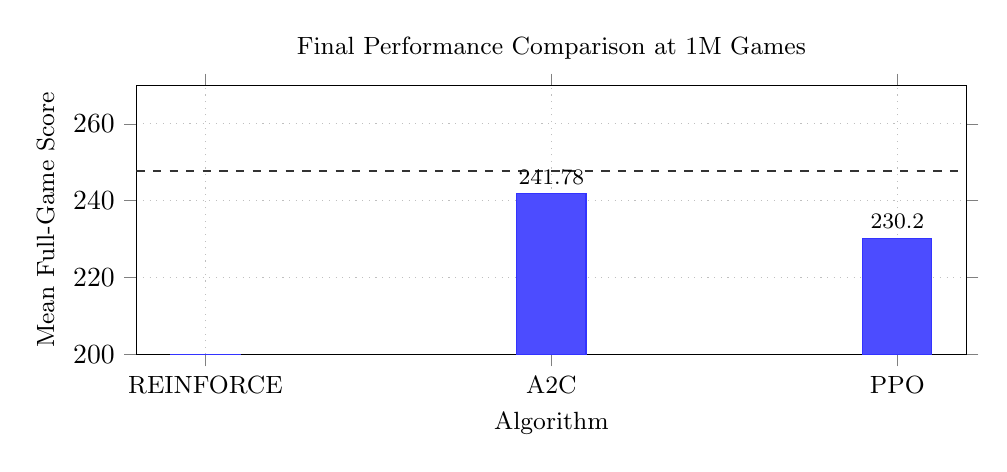
\begin{tikzpicture}
        \begin{axis}[
                ybar,
                width=\columnwidth,
                height=5cm,
                xlabel={Algorithm},
                ylabel={Mean Full-Game Score},
                title={Final Performance Comparison at 1M Games},
                symbolic x coords={REINFORCE, A2C, PPO, DP Optimal},
                xtick=data,
                xticklabel style={font=\small},
                ylabel style={font=\small},
                xlabel style={font=\small},
                title style={font=\small},
                bar width=25pt,
                ymin=200, ymax=270,
                grid=both,
                grid style={dotted},
                tick align=outside,
                nodes near coords,
                nodes near coords style={font=\footnotesize, anchor=south},
            ]

            \addplot[
                fill=blue!70!white,
                draw=blue!80,
                error bars/.cd,
                y dir=both,
                y explicit
            ] coordinates {
                    (REINFORCE, 50)
                    (A2C, 241.78)
                    (PPO, 230.20)
                };

            % Horizontal dashed line at DP optimal spanning entire graph
            \draw[dashed, black!80, thick] (rel axis cs:0,0.682) -- (rel axis cs:1,0.682);

        \end{axis}
    \end{tikzpicture}
    \caption{Final performance, mean score}
    \label{fig:final-performance-comparison}
\end{figure}